\subsection{Anomaly Detection and Fault-Domain Diagnosis}
\label{sec:real_telemetry_results}

Table~\ref{tab:binary_llo_performance} summarizes the binary anomaly-detection results under the leave-log-out protocol, which provides the strictest evaluation by assigning complete flight logs to disjoint training, validation, and test partitions. HS-AeroTS Stage 1 achieved an AUPRC of $0.6296\pm0.0023$ and an AUROC of $0.9265\pm0.0008$. At the operating threshold selected exclusively on the validation partition, its F1 score was $0.5989\pm0.0042$. The corresponding Random Forest baseline obtained an AUPRC of $0.5645\pm0.0041$.

MTCL-UAV was additionally evaluated as a recent UAV-specific deep anomaly-detection baseline using the same leave-log-out partition and the same 96-sample, 87-channel telemetry input. Its AUPRC, AUROC, and F1 were $0.4832\pm0.0082$, $0.8847\pm0.0040$, and $0.4416\pm0.0094$, respectively. Although MTCL-UAV models temporal dynamics directly through multiscale Transformer reconstruction, it did not achieve higher detection performance on UAV-SEAD under the strict cross-flight setting. This comparison should be interpreted with respect to the different learning paradigms: MTCL-UAV is trained only on normal data as an unsupervised reconstruction model, whereas HS-AeroTS Stage 1 and Random Forest are supervised binary classifiers.

\begin{table}[H]
\caption{Binary anomaly-detection performance under the leave-log-out protocol.}
\label{tab:binary_llo_performance}
\centering
\footnotesize
\renewcommand{\arraystretch}{1.12}
\begin{tabularx}{\textwidth}{@{}>{\RaggedRight\arraybackslash}p{2.55cm} >{\RaggedRight\arraybackslash}X ccc@{}}
\toprule
\textbf{Method} & \textbf{Training setting} & \textbf{AUPRC $\uparrow$} & \textbf{AUROC $\uparrow$} & \textbf{F1 $\uparrow$}\\
\midrule
MTCL-UAV & Unsupervised reconstruction & $0.4832\pm0.0082$ & $0.8847\pm0.0040$ & $0.4416\pm0.0094$\\
Random Forest & Supervised & $0.5645\pm0.0041$ & $0.9137\pm0.0042$ & $0.5553\pm0.0093$\\
HS-AeroTS Stage 1 & Supervised & $\mathbf{0.6296\pm0.0023}$ & $\mathbf{0.9265\pm0.0008}$ & $\mathbf{0.5989\pm0.0042}$\\
\bottomrule
\end{tabularx}
\par\vspace{2pt}{\scriptsize Values are mean $\pm$ standard deviation over five random seeds. Threshold-dependent metrics use operating points selected on the validation partition. MTCL-UAV follows a normal-only reconstruction setting and is therefore not directly equivalent to the supervised classifiers in training supervision.}
\end{table}

Conditional fault-domain diagnosis remained comparatively stable under strict flight-level separation. When evaluated only on anomalous windows with explicit domain labels, the Stage 2 LightGBM classifier achieved a Macro-F1 of $0.9041\pm0.0029$ and a Balanced Accuracy of $0.8876\pm0.0040$ under leave-log-out evaluation. The corresponding Random Forest classifier achieved a Macro-F1 of $0.8741\pm0.0028$. These results indicate that the four annotated fault domains remain distinguishable across unseen flight logs once anomalous windows are supplied to the diagnostic stage.

Figure~\ref{fig:protocol_robustness} compares the three data-partition protocols and shows that detection performance is more sensitive to data isolation than conditional fault-domain diagnosis. Stage 1 AUPRC decreased from $0.7522\pm0.0039$ under the fixed chronological protocol to $0.6006\pm0.0062$ under the purged protocol and recovered to $0.6296\pm0.0023$ under leave-log-out evaluation. In contrast, Stage 2 Macro-F1 was $0.8980\pm0.0020$ under the fixed chronological protocol, $0.7944\pm0.0049$ after boundary purging, and $0.9041\pm0.0029$ under leave-log-out evaluation. The protocol dependence of Stage 1 therefore constitutes the main performance bottleneck in the complete diagnostic chain.

The effect of Stage 1 gating becomes more apparent on the complete five-class task. Under leave-log-out evaluation, the hierarchical Cascade achieved a Macro-F1 of $0.5962\pm0.0048$, whereas the Direct Five-Class classifier achieved $0.6092\pm0.0043$. The paired Direct-minus-Cascade difference was 0.0130, with a flight-log bootstrap 95\% confidence interval of $[-0.0282, 0.0438]$. Since the interval includes zero, the results do not establish a stable predictive advantage for either formulation. The hierarchical design is therefore evaluated primarily as an explicit diagnostic organization that separates anomaly screening from fault-domain interpretation, rather than as a mechanism guaranteed to improve five-class predictive accuracy.

\begin{figure}[H]
    \centering
    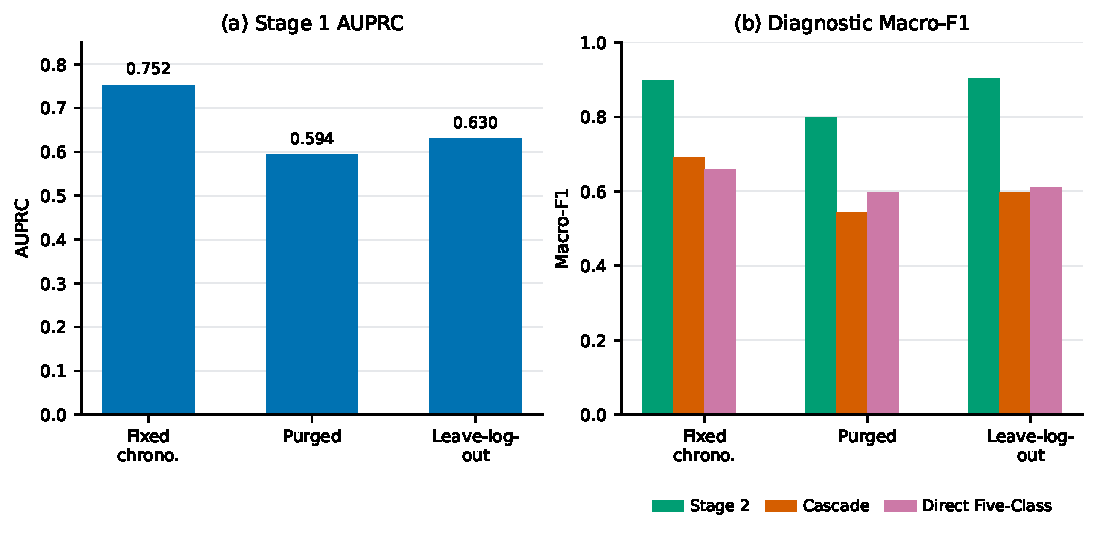
\includegraphics[width=\textwidth]{figures/figure_3_protocol_robustness.pdf}
    \caption{Performance under fixed chronological, purged, and leave-log-out protocols. Error bars show standard deviations across five model seeds. Purging reverses the mean ordering of Cascade and Direct Five-Class Macro-F1, while paired confidence intervals include zero under the stricter protocols.}
    \label{fig:protocol_robustness}
\end{figure}
